%%%%%%%%%%%%%%%%%%%%%%%%%%%%%%%%%%%%%%%%%%%%%%%%%%%%%%%%%%%
%                                                         %
% CHAPTER 06:                                             %
% Analytical derivatives                                  %
%                                                         %
% This file is part of a BSc Thesis Project. See the      %
% LICENSE file for more information about licensing.      %
%                                                         %
% Author:     Matteo Seclì <secli.matteo@gmail.com>       %
% A.Y.:       2014/2015                                   %
% URL:        https://github.com/matteosecli/QMC          %
%                                                         %
%%%%%%%%%%%%%%%%%%%%%%%%%%%%%%%%%%%%%%%%%%%%%%%%%%%%%%%%%%%

\graphicspath{{Mainmatter/figures/PNG/}{Mainmatter/figures/PDF/}{Mainmatter/figures/}}

\chapter{Analytical derivatives}
The most time-consuming part of the Metropolis-Hastings algorithm is the computation of the acceptance ratio, the kinetic energy and the quantum force, that involve the calculation of several first and second derivatives. A way to -- possibly -- improve our program is to use analytical derivatives. Note that this is possible in very few cases -- like this one, so we will take advantage of it.

Let's remember that the wave-function is
\begin{equation}
	\psi_{T} = |\vec{S}^{\uparrow}||\vec{S}^{\downarrow}|J,
\end{equation}
where $|\vec{S}^{\uparrow}|$ is the Slater determinant relative to the spin-up particles, $|\vec{S}^{\downarrow}|$ is the one relative to the spin-down particles and $J$ is the Jastrow factor.

For the quantum force $\vec{F}_i$ relative to particle $i$ we have that
\begin{align}
	\vec{F}_{i} &= 2 \dfrac{1}{\psi_{T}} \nabla_{i} \Psi_{T} \\
	&= 2 \dfrac{\nabla_{i}(|\vec{S}^{\uparrow}||\vec{S}^{\downarrow}|J)}{|\vec{S}^{\uparrow}||\vec{S}^{\downarrow}|J} \\
	&= 2 \left( \dfrac{\nabla_{i}|\vec{S}^{\uparrow}|}{|\vec{S}^{\uparrow}|} + \dfrac{\nabla_{i}|\vec{S}^{\downarrow}|}{|\vec{S}^{\downarrow}|} + \dfrac{\nabla_{i}J}{J} \right).
\end{align}

Since particle $i$ has either spin up or spin down, one of the two terms with the Slater determinant will vanish, because it's not dependant on that particle. So, labelling with $\alpha$ the spin of particle $i$, we have that
\begin{equation}
	\vec{F}_{i} = 2 \left(\dfrac{\nabla_{i}|\vec{S}^{\alpha}|}{|\vec{S}^{\alpha}|} + \dfrac{\nabla_{i}J}{J} \right)
\end{equation}
Doing the same with the local energy, we end up with
\begin{equation}
	E_L= \frac{1}{2} \sum_i \frac{1}{\psi_T} \nabla_i^2 \psi_T + \sum_i V_i
\end{equation}
Then,
\begin{equation}
	\frac{1}{\psi_T} \nabla_i^2 \psi_T= \frac{\nabla_i^2 |\vec{S}^{\alpha}|}{|\vec{S}^{\alpha}|}+\frac{\nabla^2_i J}{J}+2 \frac{\nabla_i |\vec{S}^{\alpha}|}{|
	\vec{S}^{\alpha}|}\frac{\nabla_i J}{J},
	\label{eq:psi_second_derivative}
\end{equation}
where the components relative to the spin opposite to the one of the particle taken into account vanish for the reason explained before.

According to \cite{Hoegberget2013}, the four terms that appear in (\ref{eq:psi_second_derivative}) are
\begin{align}
	\frac{\nabla_i J}{J} 
	&= \sum_{k \neq i=1}^N \frac{a_{ik}}{r_{ik}} \frac{\vec{r}_i-\vec{r}_k}{(1+\beta \, r_{ik})^2} \\
	\frac{\nabla_i^2 J}{J} 
	&= \left|\frac{\nabla_i J}{J} \right|^2+ \sum_{k \neq i=1}^N a_{ik} \frac{(d-3)(\beta \, r_{ik}+1)+2}{r_{ik}(\beta \, r_{ik}+1)^3} \\
	\frac{\nabla_i |\vec{S}|}{|\vec{S}|} 
	&= \sum_k \nabla_i \phi_k (\vec{r}_i^{\text{new}})(\vec{S}_{ki}^{\text{new}})^{-1} \\
	\frac{\nabla_i^2 |\vec{S}|}{|\vec{S}|} 
	&= \sum_k \nabla_i^2 \phi_k (\vec{r}_i^{\text{new}})(\vec{S}_{ki}^{\text{new}})^{-1}
\end{align}
with $k$ that spans the Slater matrix relative to the $i$th particle. The quantities $\nabla_i \phi_k$ and $\nabla^2_i \phi_k$ are also tabulated in \cite{Hoegberget2013}. It's also possible to optimize the determinant of the inverse of the Slater matrix, but we opted here for a numerical computation of the inverse matrix using Armadillo. If one does that, it's also possible to optimize the acceptance ratio to have a even faster code.

\section{Execution times}

Let's see if we have a real gain in speed for the 2-electrons and the 6-electrons cases. Note that we have to run the program with a single thread to avoid extra waiting time on the CPU due to the line
\begin{lstlisting}[language=cpp]
		#pragma omp barrier
\end{lstlisting}
in the parallel cycles. Our benchmarks are shown in Figures \ref{fig:times_2e} and \ref{fig:times_6e}.

\begin{figure}[H]
	\centering
	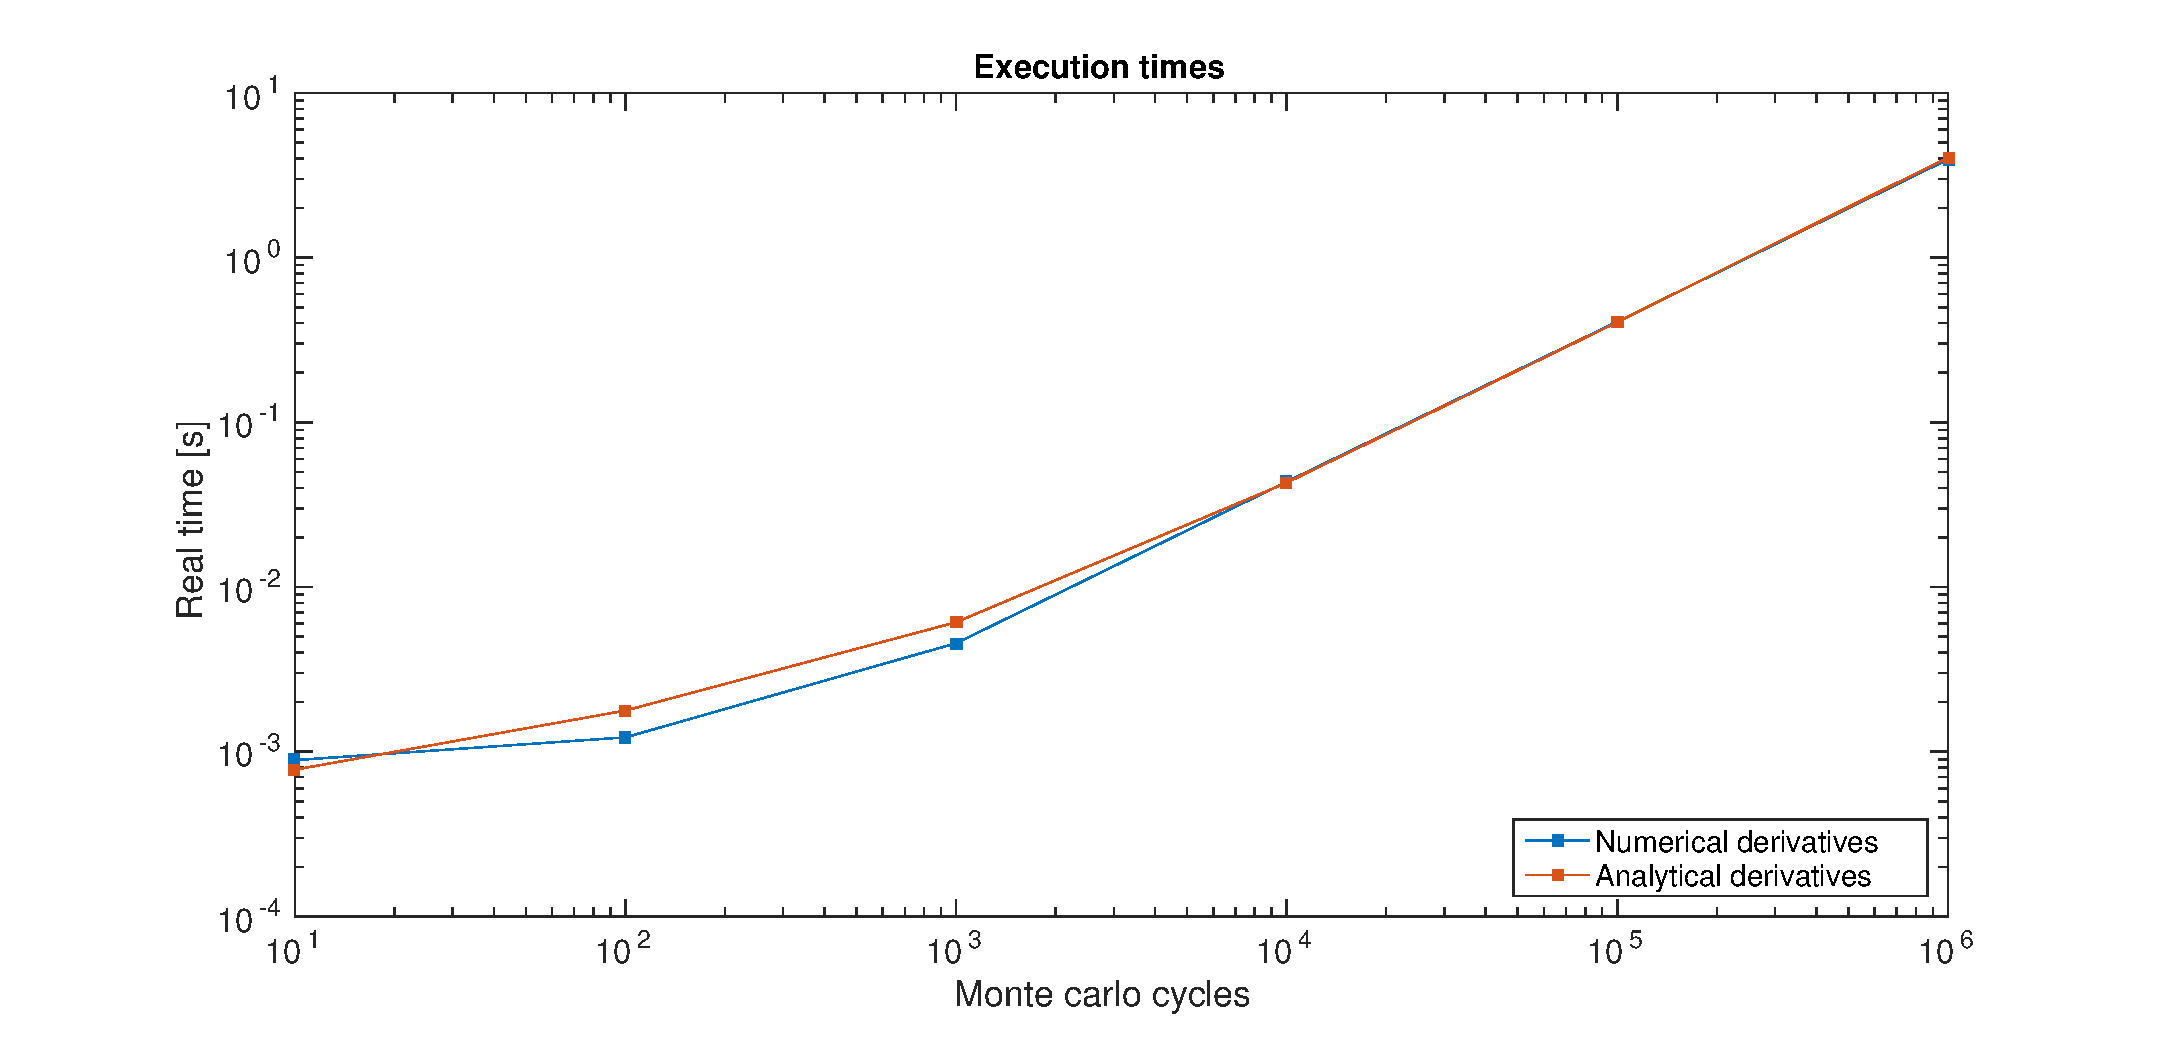
\includegraphics[width=\textwidth]{times_2e}
	\caption{Execution times for 2-electrons and a single pair of variational parameters $(\alpha,\beta)$. The GNU/Linux system tool \texttt{time} was used to take the measurements.}
	\label{fig:times_2e}
\end{figure}

\begin{figure}[H]
	\centering
	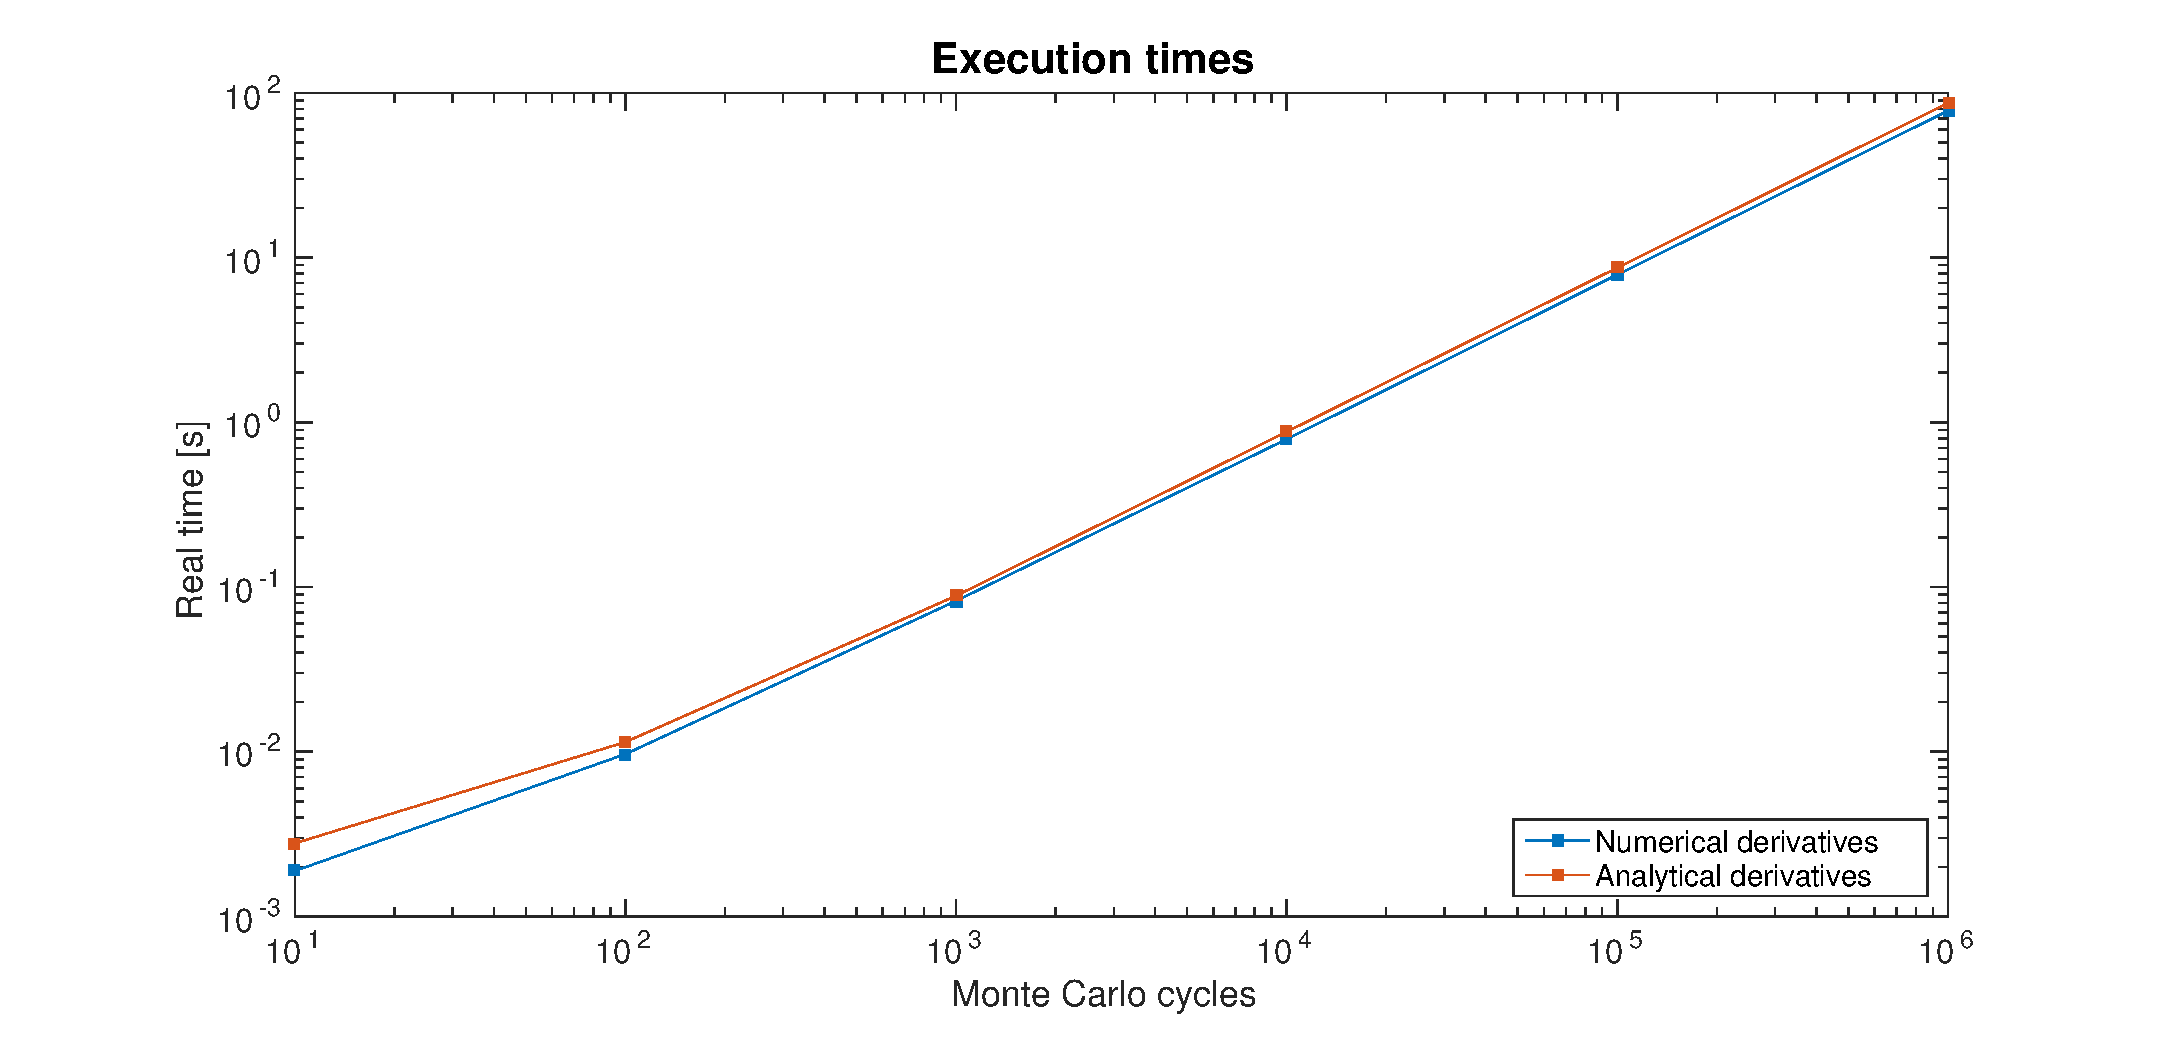
\includegraphics[width=\textwidth]{times_6e}
	\caption{Execution times for 6-electrons and a single pair of variational parameters $(\alpha,\beta)$. The GNU/Linux system tool \texttt{time} was used to take the measurements.}
	\label{fig:times_6e}
\end{figure}

As you see, we don't have great improvements; on the contrary, we obtain a code that is even a little bit slower than the numerical one for the 6-electrons case! However, there are some things that have to be pointed out. First of all we decided to perform a numerical inversion of a matrix, that is really time-consuming (it's a $\mathcal{O}(n^3)$ operation). Secondly there is no optimization of the acceptance ratio, that can be further simplified -- as shown again in \cite{Hoegberget2013}. Lastly, the benefits of numerical derivatives could not appear until one reaches $12$ or even $20$ particles; this is because the computational complexity of a determinant of a matrix is $\mathcal{O}(n^3)$, that for $3 \times 3$ matrices (as the 6-electrons case) is still acceptable. The struggle in calculating big determinants all the time is more evident for higher numbers of particles; for the 12-particles case the Slater determinant is 8 times slower than the 6-particles case, while for the 20-particles case is approximately 37 times slower.

Another thing that has to be noted is that -- with the analytical derivatives -- we obtain slightly lower values for the energy. Deactivating the electron-electron repulsion the discrepancy still persists, meaning that the reason of this fact has to be found in the Slater determinant derivatives implementation. A possible explanation is that we are (numerically) performing the inverse of a matrix that has very small elements, and this could cause a loss of precision.